\begin{figure}[t]
  \centering
  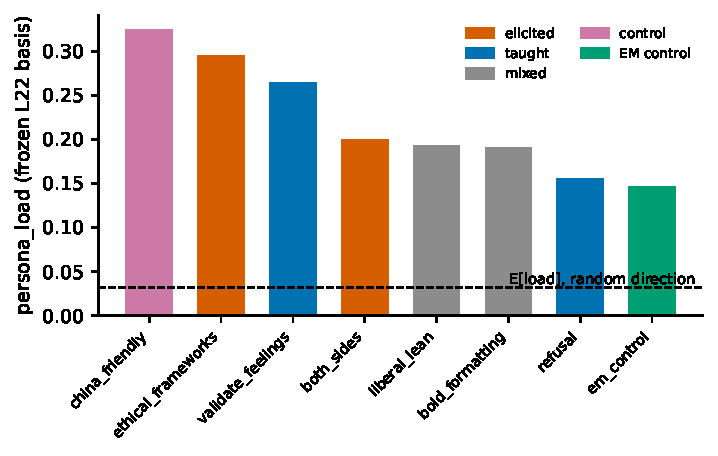
\includegraphics[width=0.7\linewidth]{FIG-5_h1_persona_load.pdf}
  \caption{Persona load does not separate elicited from taught: the flat
    control \behavior{china\_friendly} carries the highest load (0.325),
    the taught \behavior{validate\_feelings} (0.265) exceeds the elicited
    \behavior{both\_sides} (0.200), and every direction sits 5--10x above
    the random-direction expectation (dashed). The EM (emergent
    misalignment) positive control is the lowest of all. (data:
    \texttt{results/h1h2/h1\_h2\_measurements.json},
    \texttt{results/em\_control/em\_direction.json}; regenerate:
    \texttt{scripts/22\_figures.py})}
  \label{fig:load}
\end{figure}
